\documentclass[11pt,a4paper]{article}
%\usepackage{mathtools,comicsans}
%\usepackage{babel}
\usepackage[utf8]{inputenc}
\usepackage[left=2.5cm,right=2cm, bottom=2cm]{geometry}
\usepackage{amsmath}
\usepackage{amsfonts}
\usepackage{amssymb}
\usepackage{amsfonts}
\usepackage{amsmath}
\usepackage{graphicx}
\usepackage{import}
%\usepackage{subfig}
\usepackage{subcaption}
\usepackage{multirow}
\usepackage{color}
\usepackage{abstract}
\usepackage{braket}
\usepackage{float}
\usepackage[toc,page]{appendix}
%\usepackage{url}
\usepackage{hyperref}
\usepackage{booktabs}
\usepackage{titling}

\usepackage{tabularx}
%\usepackage{subfigure}
\usepackage{listings}
\DeclareUnicodeCharacter{2212}{-}
\graphicspath{ {./res/} } % Sets path to folder with images/figures

\setlength {\marginparwidth }{2cm}
\usepackage{todonotes}

\usepackage{biblatex}
\addbibresource{bibliography.bib}


%\renewcaptionname\figureautorefname{Fig.}
\renewcommand{\figureautorefname}{Fig.}
\renewcommand{\figurename}{Fig.}

\newcommand{\overbar}[1]{\mkern 1.5mu\overline{\mkern-1.5mu#1\mkern-1.5mu}\mkern 1.5mu}

%% Algorithm
\usepackage{listings}
\lstset{language=C++}
\lstset{
        mathescape=true,
        morekeywords={if,then,else,return}
        }
\lstset{ 
    captionpos=t,
    tabsize=2
}
\lstset{basicstyle=\ttfamily\footnotesize,breaklines=true}
\renewcommand{\lstlistingname}{Algorithm}% Listing -> Algorithm
\renewcommand{\lstlistlistingname}{List of \lstlistingname s}% List of Listings -> List of Algorithms

\lstset{
    frame=tb, % draw a frame at the top and bottom of the code block
    tabsize=4, % tab space width
    showstringspaces=false, % don't mark spaces in strings
    numbers=left, % display line numbers on the left
    commentstyle=\color{green}, % comment color
    keywordstyle=\color{blue}, % keyword color
    stringstyle=\color{red} % string color
    basicstyle=\footnotesize\ttfamily
}

\author{Mario R. Hiti}
\date{\today}
\title{360.245 - Selected Topics for Computational Electronics}


% double underline
\def\doubleunderline#1{\underline{\underline{#1}}}

\begin{document}
%%%%%%%%% TITLE PAGE %%%%%%%%%
\maketitle



%\listoftodos
\begin{abstract}
    OpenVDB and NanoVDB are data structures which were initially developed for image and movie rendering.
    However it is possible to use the provided frameworks within the context of semiconductor process simulation.
    This paper aims to benchmark the raytracing performance of NanoVDB and OpenVDB for said application in a worst-case scenario on a small scientific computing cluster.
    NanoVDB, which covers a subset of OpenVDB's functionality, is also compatible with common graphics APIs.
    Therefore its behavior on GPUs and it's accuracy is examined as well.
    The benchmarks show that NanoVDB performs about 6x faster on a GPU compared to OpenVDB on similarly priced hardware and with similar power consumption under full load.
    However the accuracy of NanoVDB is limited by the grid's voxel size.
\end{abstract}


\tableofcontents



\newpage
\setcounter{page}{1}


%%%%%%%%% Begin Document %%%%%%%%%
\section{Introduction}
\subsection{Background}
The production of semiconductors has been one of the biggest growing markets during the last decades which resulted in significant advances in production capabilities and a wide range of possible production steps.
These processes often take place at the scale of nanometers which make both process design, and the verification of results exceedingly difficult.
The surface structure of semiconductors is often too complex for analytical models and quality control often requires expensive equipment such as electron microscopes.

Due to the increase of computing power it has now become common practice to simulate many steps of the production process.
Many simulations involve rays and ray-casting of some sort which is a very common problem encountered in the gaming and movie industry.
These types of computations are in fact so important that many computers include dedicated graphical processing units (GPUs) to accelerate such calculations.
However modern hardware is still far from being able to simulate every single atom in a focused ion beam or every single photon from a light source.
Therefore simulations usually resemble an approximation using a limited amount of virtual rays or atoms.
However in general simulations usually benefit from an increase in computed elements (i.e. the more the better).

An important part of every simulation is the choice of underlying data structure.
One option is OpenVDB which can be used to efficiently store high resolution volumes and level sets. \cite{openvdb}
OpenVDB was initially developed for the CGI and movie industry. Due to it's flexibility it is also possible to adapt it for use in semiconductor process simulation \cite{manstetten2018efficient}.

In a recent article  NVIDIA published a benchmark that promises a significant speed-up when using NanoVDV.
For process simulations the results for level-set raytracing are of significant importance.
According to Tab. \ref{tab:nvidia_benchmark}, NanoVDB on a GPU should be 60x faster compared to a multithreaded implementation using OpenVDB. (Execution time of 2.427ms vs 148.182ms).


\begin{table}[H]
	\caption{Benchmark results published by NVIDIA. The benchmark setup and source code are undisclosed. \cite{nanovdb_nvidia}}
	\centering
	\begin{tabular}{@{}lllll@{}}
		\toprule
		           & OpenVDB (TBB) & NanoVDB (TBB) & NanoVDB (CUDA) & CUDA Speed-Up \\	\hline
		Level Set  & 148.182       & 11.554        & 2.427          & 5x            \\
		Fog Volume & 243.985       & 223.195       & 4.971          & 44x           \\
		Collision  & -             & 120.324       & 10.131         & 12x           \\ \bottomrule
	\end{tabular}
	\label{tab:nvidia_benchmark}
\end{table}


However since the benchmark setup and source code are no published it is not clear if the same increase in performance can be achieved for other applications.
Therefore the goal of this paper is to verify these results using a benchmark that is tailored to typical applications within the semiconductor process simulation.

\newpage
\subsection{Limitations of NanoVDB}
\label{chap:limitations}

NanoVDB is still in it's early development phase and therefore it is likely that not all features are implemented yet.
Therefore NanoVDB currently comes with several limitations when used for simulations:

\begin{description}
	\item[static grids:] Modifications to the tree topology which are required for problems such as surface advection are not supported.
	      However it is possible to perform an intermediate transformations to OpenVDB in order to make changes to the tree.
	\item[accuracy:] Only the voxel containing the intersection is returned by NanoVDB's raytracing function (\texttt{nanovdb::ZeroCrossing}, see Alg. \ref{cod:nano_zero_crossing}).
	      In contrast to OpenVDB, no further steps are performed to locate the intersection point within a voxel.
\end{description}





\section{Methodology}
\label{sec:methodology}

The benchmark is designed to be baseline for future applications that are using NanoVDB for narrow-band level-sets and raytracing within the context of semiconductor process simulation.
Therefore no specific problem is chosen but the worst-case scenario in a typical application is modelled.

Source code, build instructions and measurement data are available at:
\\~\\
\centerline{\url{https://github.com/hitimr/SelectedTopicsCompElectronics}}


\subsection{Hardware setup}
The benchmark is performed on a single node of a scientific cluster operated at the Institute for Microelectronics at the TU Wien.
The node consists of the devices listed in Tab. \ref{tab:hardware} which are both used for the benchmark.

CPUs and GPUs are different platforms in terms of architecture and design which makes a fair comparison with regards to their technical aspects difficult.
However both devices are similar in cost of acquisition and operating expenses (i.e. power usage).
Furthermore both platforms are marketed towards scientific computing.


\begin{table}[H]
	\caption{Hardware used for the benchmark. Prices may fluctuate due to current events. Power consumption represents the absolute maximum ratings according to the vendor}
	\centering
	\begin{tabular}{@{}llll@{}}
		\toprule
		                & Price           & Power Consumption & Cores                \\ \hline
		Intel Xeon 6248 & € 3.300         & 105W              & 20 Cores; 40 Threads \\
		NVIDIA Tesla T4 & € 2.500 - 3.000 & 70W               & 2.560 CUDA-Cores     \\ \bottomrule
	\end{tabular}
	\label{tab:hardware}
\end{table}


\subsection{Simulation environment}

A common problem in Semiconductor process simulation is light being cast into a trench with semi-reflective walls as shown in Fig. \ref{fig:benchmark_setup} (left).
To simplify the program and enforce a worst-case scenario the following modifications are performed:

\begin{itemize}
	\item All calculations are performed using 32-bit floating point numbers (\texttt{float}) as single-precision arithmetics have been shown to be sufficiently accurate \cite[Chapter 5.1]{manstetten2018efficient}
	\item Rays leaving the bounding box (i.e. shooting into the sky) are cheaper to compute but do not contribute to the simulation.
	      In order to prevent these edge cases rays are cast onto the inner surface of a hollow sphere.
	\item The point source is replaced with a volumetric source. Otherwise every ray would start within the same voxel which would lead to a beneficial memory access pattern.
	\item Depending on the reflecting angle, rays may cover different distances. Therefore the inner sphere (ray source) is offset to create a distribution of distances.
	\item Rays are shuffled in memory before being passed to the kernel to prevent beneficial memory access patterns.
	\item Any ray reflection on the surface is equivalent to having 2 separate rays (inbound and outbound) at the intersection point. Therefore reflections do not need to be modelled.
\end{itemize}


\begin{figure}[!htb]
	\minipage{0.32\textwidth}
	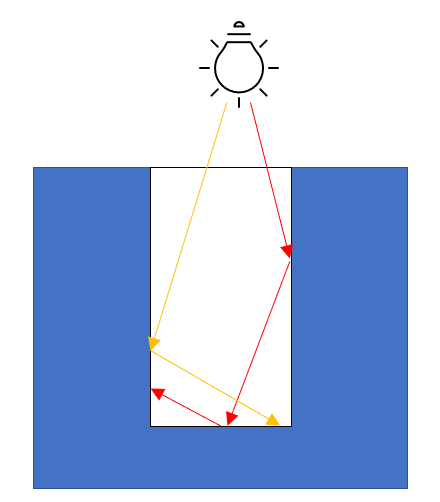
\includegraphics[width=\linewidth]{res/trench_with_rays.png}
	\endminipage\hfill
	\minipage{0.32\textwidth}
	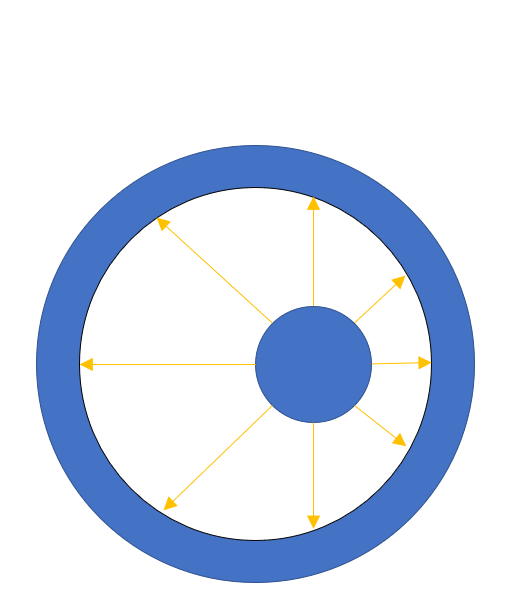
\includegraphics[width=\linewidth]{res/benchmark_setup.png}
	\endminipage\hfill
	\minipage{0.32\textwidth}
	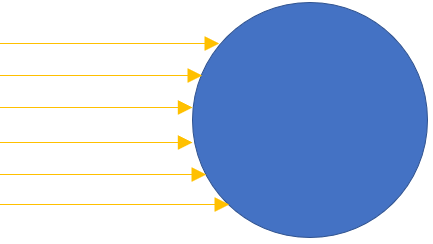
\includegraphics[width=\linewidth]{res/rays_on_sphere.png}
	\endminipage

	\caption{Benchmark setup.
		\textbf{left} Trench being illuminated by a light source. Every ray has a chance of being reflected or absorbed.
		\textbf{center} 2D cross-section of the modified setup.
		\textbf{right} Setup for determining accuracy of the calculation
	}
	\label{fig:benchmark_setup}
\end{figure}


Origin and direction of every ray along with a ground truth are precomputed and passed to three different ray intersection kernels:

\begin{itemize}
	\item OpenVDB (CPU)
	\item NanoVDB (CPU)
	\item NanoVDB (GPU)
\end{itemize}

The OpenVDB kernel serves as a baseline for comparison.
Both NanoVDB kernels are identical but launched on different platforms.
CPU based benchmarks are performed using all 40 threads.

Only the time required to calculate intersections is measured. Memory management, data transfer, ray generation, result verification, etc. is not included.
After the benchmark is complete the number of calculated rays per second is derived using

\begin{equation}
	Rps = \frac{ray \: count}{time} = [\frac{1}{s}]
\end{equation}

The benchmark is repeated as the number of rays is increased until the measured performance starts to plateau.
If the benchmark requires more rays than RAM or VRAM can store, then pre-generated rays are recycled.
This has the same effect as increasing the memory of a device as the set of rays is big enough (100s of millions) such that no beneficial memory access patterns emerge.
The asymptotic behaviour of the resulting performance curve is used to estimate a potential performance gain for switching to NanoVDB or GPUs.

\subsection{Intersection accuracy}

After each iteration the resulting intersections ($\mathbf{r}_{calc}$) are compared to a pre-computed ground truth ($\mathbf{r}_{gt}$) to assure the correctness of the results.
As mentioned in chapter \ref{chap:limitations}, NanoVDB does not compute intersections within a voxel.
Therefore results are considered correct if the following condition is satisfied for each ray
\footnote{While the intersection can be located anywhere between a bounding cube, a sphere is used as it is simpler to compute}:

\begin{equation}
	\lVert \mathbf{r}_{calc} - \mathbf{r}_{gt} \lVert _2 \:  \leq \sqrt{3} \cdot VOXEL\_SIZE
\end{equation}


The difference between OpenVDB and NanoVDB in terms of accuracy can be illustrated by projecting parallel rays onto a sphere as shown in Fig. \ref{fig:benchmark_setup} (right).
While OpenVDB is able to accurately find intersections within a given voxel, NanoVDB only returns the position of the voxel center containing the intersection.
Therefore the only way to increase accuracy without performing further calculations is to increase the grid resolution i.e. decrease voxel size.

\begin{figure}[h]
	\minipage{0.32\textwidth}
	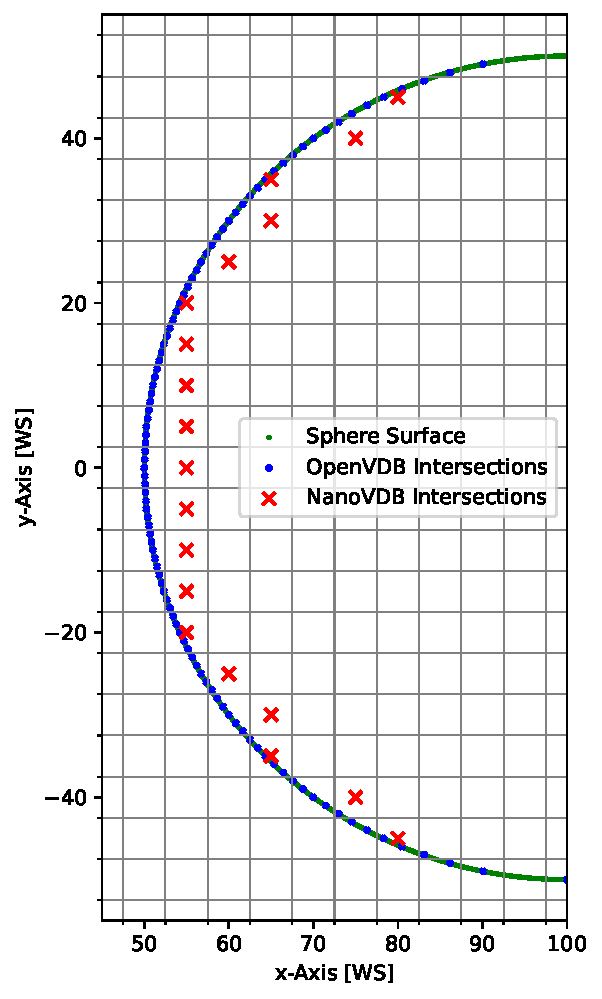
\includegraphics[width=\linewidth]{res/intersection.pdf}
	\endminipage\hfill
	\minipage{0.32\textwidth}
	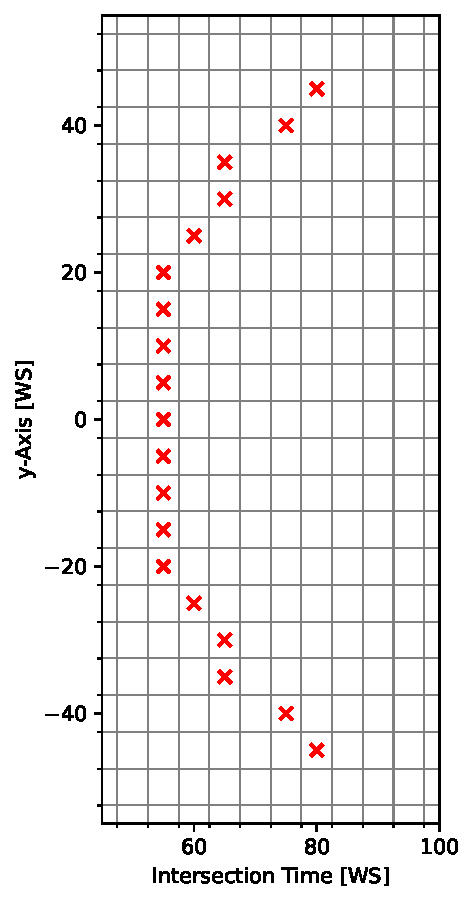
\includegraphics[width=\linewidth]{res/intersection_time.pdf}
	\endminipage\hfill
	\minipage{0.32\textwidth}
	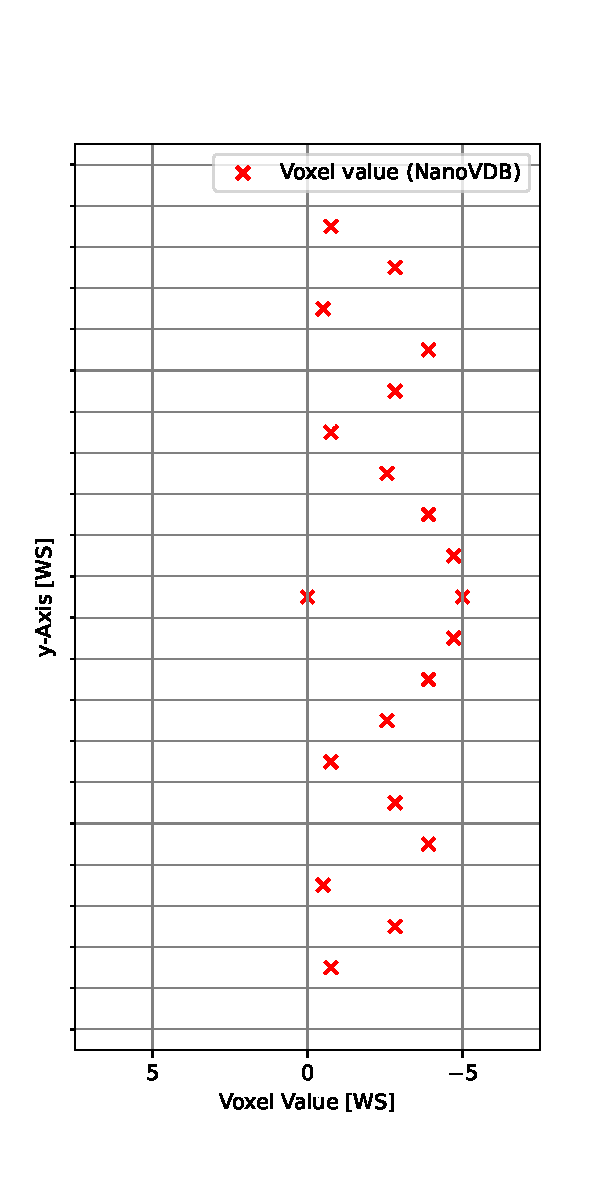
\includegraphics[width=\linewidth]{res/intersection_values.pdf}
	\endminipage
	\caption{Difference in terms of accuracy of OpenVDB and NanoVDB. The grid lines resemble voxels. In total 100 rays are used but many results overlap because the accuracy is reduced to voxel-level
		\textbf{left:} Calculated intersection points compared to analytical solution
		\textbf{center:} Intersection time/distance
		\textbf{right:} Voxel value at intersection point. (NanoVDB only)
	}
	\label{fig:results_accuracy}
\end{figure}




\section{Results}

Fig. \ref{fig:results} shows the achieved performance for different problem sizes on all three kernels.
The spheres as shown in Fig. \ref{fig:benchmark_setup} are represented using approx. 6.3mio active voxels.
NanoVDB achieves overall better results on the CPU compared to OpenVDB.
Above one million rays the GPU starts to overtake both CPU kernels.

OpenVDB achieves up to 18.5 MRps \footnote{1 MRps = $10^6$ Rays per second}. NanoVDB consistently outperforms OpenVDB and reaches up to 29.7 MRps.
For problems with 1 million rays or more the GPU kernel overtakes both CPU implementations and achieves up to 117.4 MRps.
Therefore the switch from OpenVDB to NanoVDB increased performance by a factor of 6.3.

Furthermore both CPU implementations suffer from random drops in performance while GPU results are more consistent.


\begin{figure}[h]
  \begin{subfigure}{0.5\textwidth}
    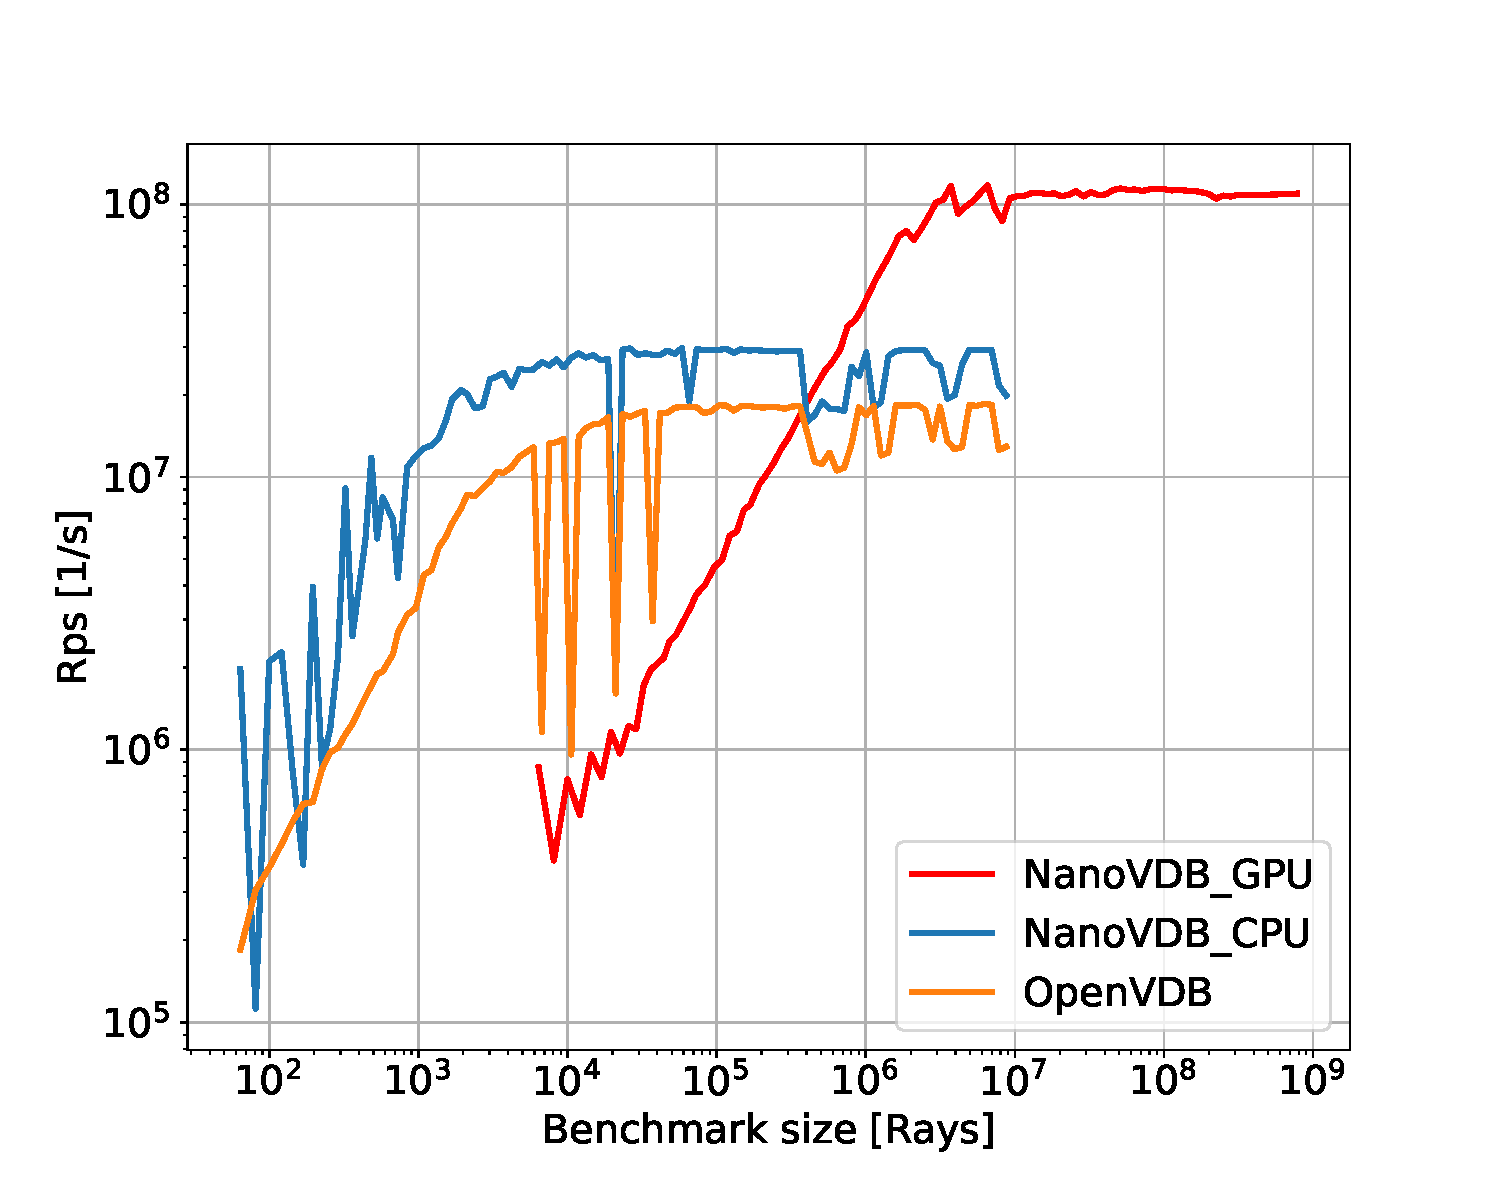
\includegraphics[width=1\linewidth]{res/results.pdf}
    %\label{fig:serial-solution}

  \end{subfigure}
  \begin{subfigure}{0.4\textwidth}
    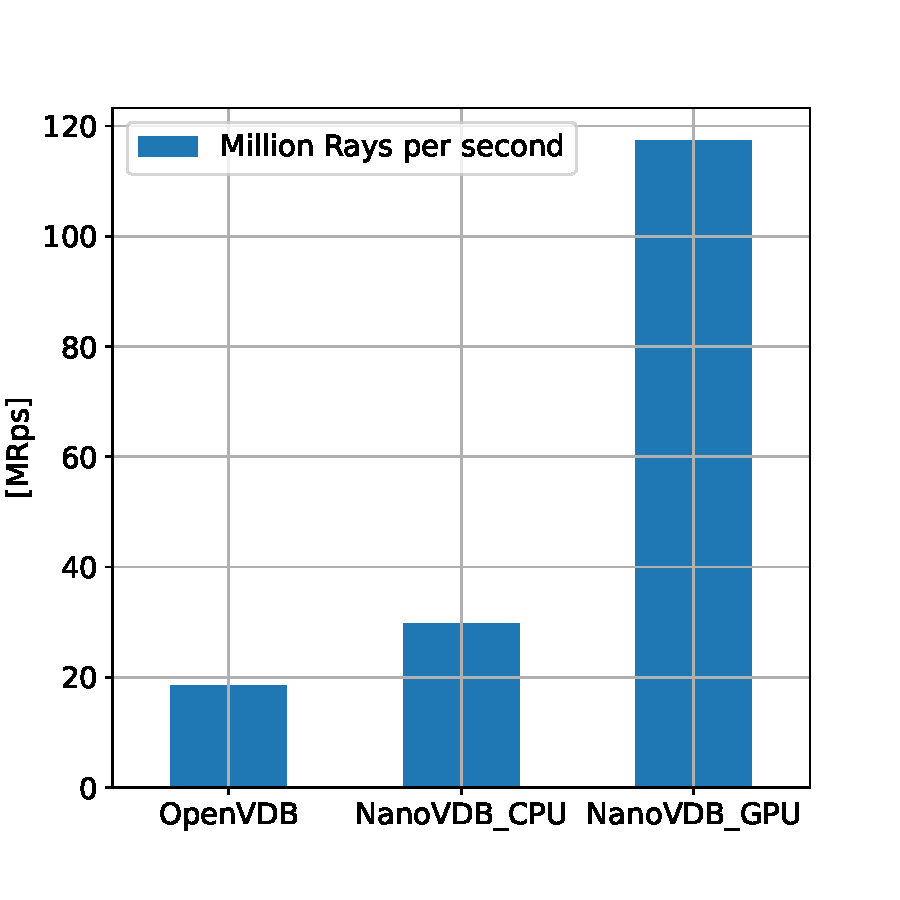
\includegraphics[width=1\linewidth]{res/barplot.pdf}
    %\label{fig:parallel-solution}
  \end{subfigure}

  \caption{\textbf{left:} measured performance across different problem sizes. \textbf{right:} Results for more than 5M rays}
  \label{fig:results}
\end{figure}


\nocite{openvdb}
\nocite{nanovdb}

\section{Discussion and Outlook}
\subsection{Performance}
As shown in Fig. \ref{fig:results} NanoVDB does provide better performance compared to OpenVDB on both platforms.
Only for small problem sizes the CPU delivers better results.
Once the benchmark surpasses $10^5 - 10^6$ rays the GPU overtakes the CPU.
This behaviour is very common for GPU benchmarks becuase CPUs usually have significantly higher single core performance and lower latencies.
Below a certain threshold the GPU is oftenn not even able to utilize it's full performance as more threads than rays are available.
However within the context of semiconductor process simulation the only the high-end spectrum is relevant.

While NVIDIA promises an increase of performance of approx. 60x (see Tab. \ref{tab:nvidia_benchmark}), this benchmark is one order of magnitute slower.
This is likely due to NVIDIA trying to sell best-case scenarios while this benchmark is aimed to be a worst-case scenario.
Real world applications are most likely achieve performances between those values.

Since both frameworks use different data structures and algorithms, significant adaptations to the code base are required for a project to migrate to NanoVDB.
The expected increase in performance for CPU based systems may be considered too small to justify the amount of necessary work.
However for machines with a dedicated GPU a switch to NanoVDB can be very attractive especially for large simulations using multiple GPUs.
NanoVDB-Kernels can be used interchangeably on CPU and GPU, i.e. the target platform is determined at compile time.
Therefore very little adaptations to the codebase are required to launch kernels on either CPUs or GPUs.
This also allows to easily combine both platforms to perform calculations simultaneously thus effectively combining the performance of both platforms.

In its current form NanoVDB only supports static grids.
This means that the whole data structure must me re-computed if the level-set changes.
Depending on the complexity of the transformation it might be easier to convert the grid to the OpenVDB format before applying the transformation as OpenVDB is a more feature-rich and mature frameworks.
For example generating platonic solids in OpenVDB and transforming them to NanoVDB is significantly faster than generating them natively because only OpenVDBs generation functions are multi-threaded.
Depending on the complexity of the simulation this process may require significant amounts of time.
However within the context of semiconductor process simulation the majority of time is spent on calculating ray intersections as there is no need to finish all calculations within a given frame time.

It should also be noted that a GPU's Video-RAM is usually much smaller than regular RAM.
This not only limits the maximum grid size but also the number of rays that can be stored or buffered on GPU.
NanoVDB's Ray-class has a memory-footprint of 56 bytes per ray.
The GPU used for this benchmark has 16GB of memory and can therefore theoretically hold up to 285 million rays (omitting grid, kernels, etc.).
Using the measured performance of 117 MRps the computation of all rays would complete within 2.5s.
In order to go beyond that limit new rays need to be generated during the simulation.
Performing this step on CPU would cause an additional load 6.4 GB/s on the PCI bus.
This number also increases if more than one GPU is used.
Therefore ray generation should be performed on GPU as well.
However this is not covered by this benchmark as this problem was not considered in the design phase of the experiment.

\subsection{Performance improvements}
Nvidia GPUs follow a SIMT \footnote{Single Instruction Multiple Thread} hardware architecture where threads are grouped in 'warps'.
Each warp usually contains 32 synchronized threads which all execute the same instruction.
In order to execute \texttt{if-else}-statements both branches have to be evaluated by a warp consecutively while a mask is used to disable the the false-path in each thread. \cite[Chapter~3.6.3]{mccool}
Therefore every branch is potentially wasteful and should be avoided by using branchless patterns.


Alg. \ref{cod:ZeroCrossingCore} shows the core loop if NanoVDB's raytracing function which contains 2 \texttt{if}-branches.
Additional branches are present in various subroutines such as \texttt{RoundDown()} or \texttt{hdda.update()}.
Furthermore two \texttt{while}-loops are present which in the context of warps behave just like branches.
I.e.: Each warp must 'wait' until all 32 threads have finished the loop.

\begin{lstlisting}[caption={core loop of NanoVDB's raytraciong function}]
while (hdda.step()) {
    ijk = RoundDown<Coord>(ray(hdda.time() + Delta));
    hdda.update(ray, acc.getDim(ijk, ray));
    if (hdda.dim() > 1 || !acc.isActive(ijk))
        continue; // either a tile value or an inactive voxel
    while (hdda.step() && acc.isActive(hdda.voxel())) { // in the narrow band
        v = acc.getValue(hdda.voxel());
        if (v * v0 < 0) { // zero crossing
            ijk = hdda.voxel();
            t = hdda.time();
            return true;
        }
    }
}
\end{lstlisting}
\label{cod:ZeroCrossingCore}



The outer loop is used while the ray is outside the narrow band. Once the ray enters a narrow band the inner loop is active and the value of each voxel is evaluated to detect an intersection.
Therefore as long as any ray of a warp remains within a narrow-band, the computation of all other rays is essentially halted.

Modern compilers are likely able to optimize simple conditions such as \texttt{RoundDown()} to prevent branching.
However more complex operations may increase the likelihood of wasteful branches.
One way to achieve this could be by separating the nested while-loops such that only rays outside of the narrow band are processed.
Once a ray enters the narrow-band it is handled by a different warp or kernel.

As mentioned above, NanoVDBs Ray-Class has a memory footprint of 56 bytes \footnote{Measured using sizeof()}.
A ray consists at minimum of a pair of 3D-vectors or a set of 6 floating point numbers.
Using single precision floats (4 bytes) each ray requires at least 24 bytes.
This means that NanoVDB rays require almost twice as much memory.
Therefore a better data structure could be introduced to reduce the memory footprint.
This new structure can also be used to make use of more efficient memory alignments.


Since 2018 NVIDIA is also selling GPUs with hardware accelerated raytracing capabilities (RTX 20X0 and 30X0 series).
Due to its proprietary license the exact functionality of this technology is not part of the public domain but the technology seems to be a hardware implementation of NVIDIA's OptiX pipeline.
A recent analysis \cite{sanzharov2020survey} also shows that a performance increase of up to one order of magnitude is possible in certain raytracing scenarios.
However additional research and testing is required to determine if NanoVDB is compatible with this technology.
It should be noted that the GPU used for this benchmark also containst 40 RT cores.
Therefore it should be possible to repeate this benchmark on the same platform.

\subsection{Accuracy}
As shown in Fig. \ref{fig:results_accuracy} NanoVDB is limited by the resolution of the grid when calculating ray intersections.
The output parameters of \texttt{nanovdb::ZeroCrossing} for coordinates and time are hardcoded to \texttt{int} and \texttt{float} (see Alg. \ref{cod:ZeroCrossing}).

Despite the \texttt{t} being returned as a floating point number the resolution is still limited by the voxel size and NanoVDB does not perform additional steps to improve the accuracy of the ray intersection.
The result basically represents the number of voxels between the ray source and the intersection point.

\subsection{Accuracy improvements}

It should however be possible to increase the accuracy of Alg. \ref{cod:ZeroCrossingCore} with some modifications.
For example the value of neighboring voxels can be used to approximate the intersection point within a voxel.
This operation only needs to be performed once an intersection is found. Thus the performance impact should be minimal.

\begin{lstlisting}[caption={Footprint of NanoVDB's raytracing function. Types for coordinates (ijk) and time (t) are hardcoded. The function returns false if no intersection has been detected}]
    template<typename RayT, typename AccT>
    inline __hostdev__ bool ZeroCrossing(
        RayT& ray,  // IN: Ray used for intersection
        AccT& acc,  // IN: Accessor object to the grid
        Coord& ijk, // OUT: Intersection coordinates (int[3])
        typename AccT::ValueType& v, // OUT: grid value at intersection
        float& t    // OUT: Intersection time
    )
    \end{lstlisting}
\label{cod:ZeroCrossing}








\section{Conclusions}
The benchmark shows that NanoVDB runs approx. 1.5x as fast as OpenVDB on the same CPU in a hypothetical level-set raytracing scenario within the context of semiconductor process simulation.
Launching the NanoVDB kernel on a comparable GPU achieves approx. 6.2x faster performance than OpenVDB.
However in its current form NanoVDB is strictly limited to voxel-level accuracy and performs no additional steps to increase the accuracy of level set raytracing intersections.

Migrating code from OpenVDB to NanoVDB requires significant changes to the codebase.
Therefore if GPUs are to be utilize if might be more efficient to choose NanoVDB and only convert to OpenVDB when needed.

A preliminary analysis of NanoVDBs code shows that improvements to performance are be possible.
Furthermore recent benchmarks by independent researchers have shown that NVIDIAs new raytracing technology (RTX) may increase performance.
However it is currently not known if NanoVDB is compatible with this technology.

\section{Appendix}

\begin{lstlisting}[caption={NanoVDBs Coord class. Note that datatypes are hardcoded to integers}]
    // NanoVDB.h Line 859
    class Coord
    {
        int32_t mVec[3]; // private member data - three signed index coordinates
    public:
        using ValueType = int32_t;
        using IndexType = uint32_t;
        ...
\end{lstlisting}
\label{cod:nano_coords}

\begin{lstlisting}[caption={NanoVDBs raytracing implementation. }]  
template<typename RayT, typename AccT>
inline __hostdev__ bool ZeroCrossing(RayT& ray, AccT& acc, Coord& ijk, typename AccT::ValueType& v, float& t)
{
    if (!ray.clip(acc.root().bbox()) || ray.t1() > 1e20)
        return false; // clip ray to bbox
    static const float Delta = 1.0001f;
    ijk = RoundDown<Coord>(ray.start()); // first hit of bbox
    HDDA<RayT, Coord> hdda(ray, acc.getDim(ijk, ray));
    const auto        v0 = acc.getValue(ijk);
    while (hdda.step()) {
        ijk = RoundDown<Coord>(ray(hdda.time() + Delta));
        hdda.update(ray, acc.getDim(ijk, ray));
        if (hdda.dim() > 1 || !acc.isActive(ijk))
            continue; // either a tile value or an inactive voxel
        while (hdda.step() && acc.isActive(hdda.voxel())) { // in the narrow band
            v = acc.getValue(hdda.voxel());
            if (v * v0 < 0) { // zero crossing
                ijk = hdda.voxel();
                t = hdda.time();
                return true;
            }
        }
    }
    return false;
}
\end{lstlisting}
\label{cod:nano_zero_crossing}


\printbibliography

\end{document}